\documentclass{article}
\usepackage{geometry} \geometry{margin=1in}
\usepackage{parskip}
\usepackage{ragged2e}
\usepackage{float}
\usepackage{tcolorbox}
\usepackage{amsmath, amssymb}
\usepackage{tikz} \usetikzlibrary{shapes, arrows.meta, positioning, shadows}
\usepackage{booktabs} % For professional tables
\usepackage{longtable} % For tables spanning multiple pages
\usepackage[table]{xcolor} % For colored table rows

% MANDATORY STYLE DEFINITIONS
\tikzset{
    block/.style={rectangle, draw, thick, rounded corners, fill=blue!5, align=center, minimum height=2em},
    process/.style={rectangle, draw, fill=blue!10, align=center},
    decision/.style={diamond, draw, fill=green!10, align=center, aspect=2},
    key/.style={circle, draw, minimum size=0.2cm, fill=black},
    comp/.style={draw, rectangle, minimum size=1cm},
    server/.style={draw, rectangle, minimum size=1.5cm, fill=gray!20},
    router/.style={draw, rectangle, minimum size=1cm, fill=yellow!20},
    target/.style={draw, rectangle, minimum size=1cm, fill=red!10},
    arrow/.style={thick, ->, >=stealth}
}
\raggedbottom
\tcbset{colback=blue!5, colframe=blue!40, boxrule=1pt}
\definecolor{ocu_blue}{HTML}{005691}
\definecolor{table_header}{HTML}{E0E0E0}

\title{\vspace{-3em}Cybersecurity (CSCI 2413): Mid-Term Review Companion Guide}
\author{Elite Academic Professor}
\date{}

\begin{document}
\maketitle
\thispagestyle{empty}

\section{Open-Source Intelligence (OSINT)}

Open-Source Intelligence (OSINT) is defined as the rigorous process of collecting and analyzing publicly available information to derive actionable insight and intelligence regarding a specific target. It is crucial to note that this information is gathered ethically and legally from sources that are accessible to the general public.

\subsection{OSINT Workflow and Steps}

The OSINT process follows a methodical workflow comprising five key steps:

\begin{enumerate}
    \item \textbf{Planning and Direction:} This initial phase requires establishing clear objectives by defining precisely what information is needed, why it is needed, and how it relates to the intelligence goal.
    \item \textbf{Collection:} Data gathering commences from public domains. Sources include social media, traditional media (news, books, reports), academic research, public records, government documents, and specialized forums. This step utilizes a mix of manual browsing and automated scraping methods.
    \item \textbf{Processing and Organization:} Raw data is inherently noisy. This step involves filtering the collected data, removing irrelevant information, and identifying and removing duplicate entries. Historically, this phase often relies heavily on manual human review.
    \item \textbf{Analysis and Correlation:} This is where intelligence is derived. Analysts identify patterns, relationships, and emerging trends within the processed data. Findings must be rigorously corroborated using multiple sources to ensure accuracy and reliability.
    \item \textbf{Dissemination:} The final intelligence is reported in a structured way (such as an intelligence report or a formal briefing) tailored specifically for the relevant stakeholders and decision-makers.
\end{enumerate}

\subsection{OSINT Targets}

OSINT techniques are widely applicable across various intelligence domains, targeting:\\
\begin{itemize}
    \item Individuals (e.g., background checks, digital footprints).
    \item Organizations and Businesses (e.g., competitive intelligence, supply chain monitoring).
    \item Critical Infrastructure (e.g., mapping network topography, security posture).
    \item Cybersecurity and Threat Intelligence (e.g., monitoring hacker forums, vulnerability discovery).
    \item Governments and Nations (e.g., political and economic insight).
    \item Public Health (e.g., tracking disease outbreaks, monitoring misinformation).
\end{itemize}

\subsection{Sock Puppets and Anonymity}

A \textbf{Sock Puppet} refers to a covert online account that is intentionally created and maintained not to be linked to the user's real identity. This is vital when performing SOCMINT (Social Media Intelligence). To protect the analyst's true identity, standard operational security dictates that they should utilize a \textbf{Virtual Machine (VM)} when interacting with the sock puppet account, and all traffic must be routed through a \textbf{VPN (Virtual Private Network)} to mask the geographical location and network origin.

\section{Cryptography Basics}

Cryptography is the practice and study of techniques for secure communication in the presence of adversarial behavior.

\subsection{Encryption and Decryption}

\begin{itemize}
    \item \textbf{Encryption:} This process transforms comprehensible information (Plain Text) into an unintelligible form (Cipher Text) using a mathematical \textbf{Algorithm} and a secret key. Effective security requires both the sender and receiver to agree on the algorithm and key beforehand. The goal is to make the message difficult to re-create without knowing the precise protocol and key.
    \item \textbf{Decryption:} This is the reversal of the scrambling protocol, using the corresponding key and algorithm to convert the Cipher Text back into comprehensible Plain Text.
\end{itemize}

\begin{figure}[H]
    \centering
    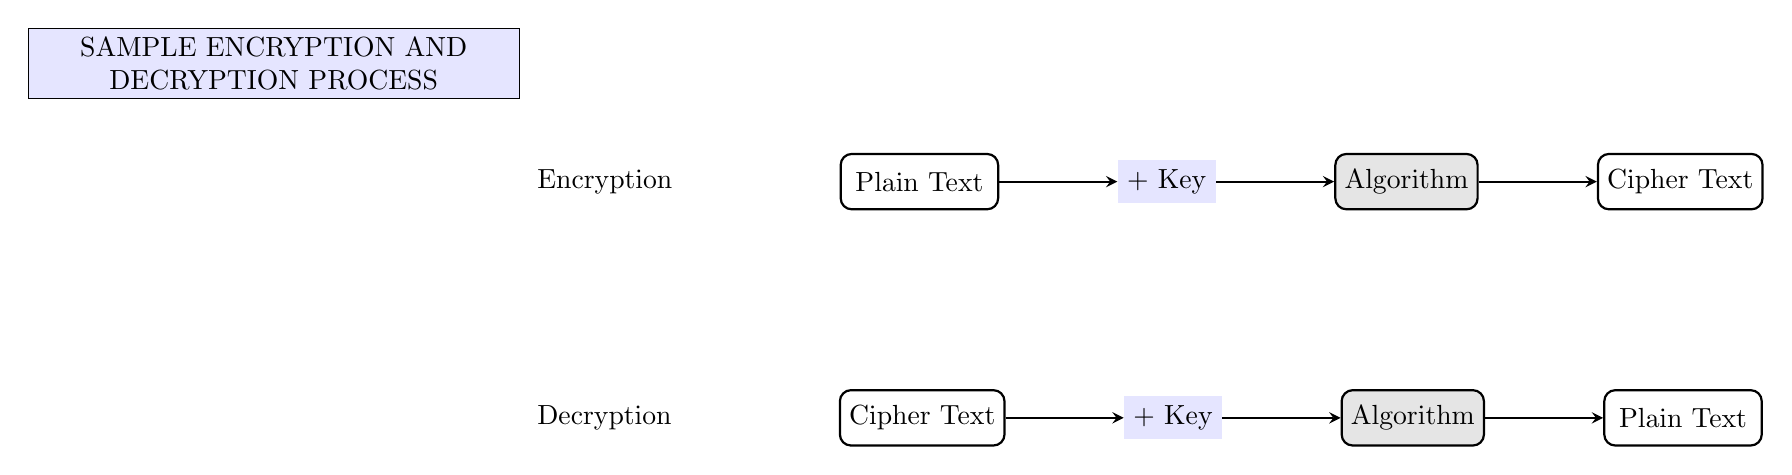
\begin{tikzpicture}[node distance=2cm, auto]
        \node (start) [process, text width=6cm] {SAMPLE ENCRYPTION AND DECRYPTION PROCESS};
        
        % Encryption Row
        \node (E_label) [right=0.1cm of start, yshift=-1.5cm, align=left] {Encryption};
        \node (E_PT) [block, right=2cm of E_label, fill=white, minimum width=2cm] {Plain Text};
        \node (E_Key) [process, right=1.5cm of E_PT, draw=none, minimum width=0.5cm] {+ Key};
        \node (E_Alg) [block, right=1.5cm of E_Key, fill=gray!20] {Algorithm};
        \node (E_CT) [block, right=1.5cm of E_Alg, fill=white, minimum width=2cm] {Cipher Text};
        
        \draw [arrow] (E_PT) -- (E_Key);
        \draw [arrow] (E_Key) -- (E_Alg);
        \draw [arrow] (E_Alg) -- (E_CT);
        
        % Decryption Row
        \node (D_label) [right=0.1cm of start, yshift=-4.5cm, align=left] {Decryption};
        \node (D_CT) [block, right=2cm of D_label, fill=white, minimum width=2cm] {Cipher Text};
        \node (D_Key) [process, right=1.5cm of D_CT, draw=none, minimum width=0.5cm] {+ Key};
        \node (D_Alg) [block, right=1.5cm of D_Key, fill=gray!20] {Algorithm};
        \node (D_PT) [block, right=1.5cm of D_Alg, fill=white, minimum width=2cm] {Plain Text};
        
        \draw [arrow] (D_CT) -- (D_Key);
        \draw [arrow] (D_Key) -- (D_Alg);
        \draw [arrow] (D_Alg) -- (D_PT);
    \end{tikzpicture}
    \caption{Conceptual flow of Encryption and Decryption}
\end{figure}

\subsection{Types of Ciphers}

Ciphers are broadly divided into two classic types:

\begin{itemize}
    \item \textbf{Transposition Ciphers:} These rearrange the letters of the plaintext without substituting them. The order is changed, but the letters themselves remain intact.
    \item \textbf{Substitution Ciphers:} These replace each letter in the plaintext with a different letter, number, or symbol.
\end{itemize}

Substitution ciphers are further classified based on key usage:

\begin{itemize}
    \item \textbf{Single/Symmetric Key Encryption:} Uses the same secret key for both encryption and decryption.
    \begin{itemize}
        \item \textit{Stream Ciphers:} Encrypt data bit-by-bit or byte-by-byte.
        \item \textit{Block Ciphers:} Encrypt data in fixed-size blocks (e.g., 64-bit blocks).
    \end{itemize}
    \item \textbf{Public/Asymmetric Key Encryption:} Uses a pair of mathematically linked keys (a public key for encryption and a private key for decryption).
\end{itemize}

\subsection{Transposition Cipher Example: Rail Fence}

The Rail Fence cipher is a simple form of transposition where the message is written in a zigzag pattern across a number of rows (the key), and the ciphertext is read row-by-row.

\begin{tcolorbox}[title=Example: Rail Fence Encryption]
Message: \textbf{Defend the east wall} (D E F E N D T H E E A S T W A L L) with a key of 3.

The letters are written:
\begin{itemize}
    \item Row 1 (Rail 1): D . . N . . E . . T . . L
    \item Row 2 (Rail 2): . E . F . D . H . E . S . W . L
    \item Row 3 (Rail 3): . . F . . T . . A . . A
\end{itemize}
(Note: Padding letters 'X' are often added to fill the last row.)

The resulting grid shown in the original slides (using padding and filling columns):
\begin{figure}[H]
    \centering
    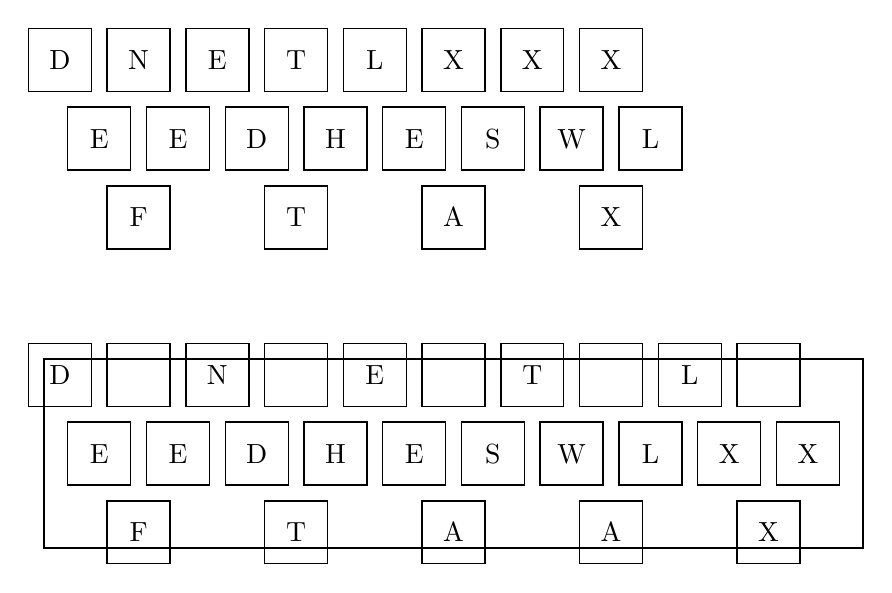
\begin{tikzpicture}[>=latex, line width=0.5pt, minimum size=0.8cm, text centered]
        \node[draw] (D) at (0, 0) {D};
        \node[draw] (N) at (1, 0) {N};
        \node[draw] (E1) at (2, 0) {E};
        \node[draw] (T1) at (3, 0) {T};
        \node[draw] (L) at (4, 0) {L};
        \node[draw] (X1) at (5, 0) {X}; 
        \node[draw] (X1) at (6, 0) {X}; 
        \node[draw] (X1) at (7, 0) {X}; 

        
        \node[draw] (E5) at (0.5, -1) {E};
        \node[draw] (E6) at (1.5, -1) {E};
        \node[draw] (D2) at (2.5, -1) {D};
        \node[draw] (H1) at (3.5, -1) {H};
        \node[draw] (E7) at (4.5, -1) {E};
        \node[draw] (S1) at (5.5, -1) {S};
        \node[draw] (W1) at (6.5, -1) {W};
        \node[draw] (L2) at (7.5, -1) {L};

        \node[draw] (F1) at (1, -2) {F};
        \node[draw] (T) at (3, -2) {T};
        \node[draw] (A2) at (5, -2) {A};
        \node[draw] (X3) at (7, -2) {X}; 
        
        % Redrawing the complex grid provided on slide 9 exactly
        \begin{scope}[shift={(0, -4)}]
        \node[draw] at (0, 0) {D};
        \node[draw] at (1, 0) {};
        \node[draw] at (2, 0) {N};
        \node[draw] at (3, 0) {};
        \node[draw] at (4, 0) {E};
        \node[draw] at (5, 0) {};
        \node[draw] at (6, 0) {T};
        \node[draw] at (7, 0) {};
        \node[draw] at (8, 0) {L};
        \node[draw] at (9, 0) {};
        
        \node[draw] at (0.5, -1) {E};
        \node[draw] at (1.5, -1) {E};
        \node[draw] at (2.5, -1) {D};
        \node[draw] at (3.5, -1) {H};
        \node[draw] at (4.5, -1) {E};
        \node[draw] at (5.5, -1) {S};
        \node[draw] at (6.5, -1) {W};
        \node[draw] at (7.5, -1) {L};
        \node[draw] at (8.5, -1) {X};
        \node[draw] at (9.5, -1) {X}; % Assume this is where the table ends visually
        
        \node[draw] at (1, -2) {F};
        \node[draw] at (3, -2) {T};
        \node[draw] at (5, -2) {A};
        \node[draw] at (7, -2) {A};
        \node[draw] at (9, -2) {X};
        
        % Ensure row boxes align and close the structure as drawn
        \draw[thick] (0-0.2, 0.2) rectangle (9.5+0.7, -2-0.2);
        
        \end{scope}
    \end{tikzpicture}
    \caption{Visual representation of Rail Fence encryption (Key=3)}
\end{figure}

The cipher text is read off row by row (DNETL... EE D H E S W L X X... F T A A X) to get: \textbf{DNETLEEDHESWLXFTAAX} (The slide shows a slightly different output: DNETLEEDHESWLXFTAAX, implying a specific sequence of padding and spaces was used).
\end{tcolorbox}

\begin{tcolorbox}[title=Example: Rail Fence Decryption]
Ciphertext received: \textbf{TEKOOHRACIRMNREATANFTETYTGHH}. Encrypted with a key of 4.

The total length is 32. Since the key is 4, we must determine how many characters belong to each rail based on the zigzag pattern (length of cycle $= 2 \times 4 - 2 = 6$). By reconstructing the pattern and placing the ciphertext sequentially into the rows, we obtain the plaintext:
\begin{center}
\textit{``They are attacking from the north''}
\end{center}
\end{tcolorbox}

\subsection{Substitution Ciphers: Caesar and Vigenere}

\subsubsection{Caesar Cipher}
The Caesar Cipher is the simplest form of substitution, known historically from written communication and warfare. It is a shift cipher where every letter in the plaintext is replaced by a letter some fixed number of positions down the alphabet.

\begin{tcolorbox}[title=Example: Caesar Cipher]
Cleartext = HELLO WORLD. Key = +2.
A becomes C, B becomes D, etc.
H (+2) $\rightarrow$ J
E (+2) $\rightarrow$ G
L (+2) $\rightarrow$ N
O (+2) $\rightarrow$ Q

Cipher Text = \textbf{JGNNQ YQTNF}
\end{tcolorbox}

The fundamental weakness of the simple Caesar cipher is that it can be easily cracked using \textbf{frequency distribution analysis}, as the relative frequency of letters (like E being the most common) remains constant across the message, only shifted.

\subsubsection{Vigenere Cipher}
The Vigenere Cipher is a polyalphabetic cipher that uses a keyword, making frequency analysis much harder because a single plaintext letter can be encrypted to multiple ciphertext letters depending on its position relative to the key.

\begin{tcolorbox}[title=Example: Vigenere Cipher]
\begin{itemize}
    \item Plaintext: ATTACKATDAWN
    \item Key: LEMON
    \item Keystream (Key Repeated): LEMONLEMONLE
    \item Ciphertext: LXFOPVEFRNHR
\end{itemize}
\end{tcolorbox}

It is crucial to note that Charles Babbage successfully \textbf{broke the Vigenere Cipher in 1854} by recognizing that if the key length could be determined (often by finding repeated sequences in the ciphertext), the long ciphertext could be treated as several interwoven Caesar ciphers, enabling frequency analysis to be applied to each column individually.

\subsection{Historical Machines: Enigma and Turing's Bombe}

\subsubsection{The Enigma Machine}
The Enigma machine was an electromechanical device created by Arthur Scherbius in 1918. Its security relied on a complex set of rotating \textbf{Rotors} that changed the substitution alphabet after every key press, a \textbf{Reflector} that sent the signal back through the rotors differently, a \textbf{Plugboard} (Steckerbrett) for extra substitution swaps, and a \textbf{Lampboard} for displaying the output. The sheer number of possible settings made brute-forcing impractical.

\subsubsection{Alan Turing and the Bombe}
Alan Turing, a foundational figure in computing and mathematics, played a pivotal role in cracking the Enigma codes during World War II. He created the first working electro-mechanical device known as the \textbf{Bombe} in the 1940s. The Bombe worked by cycling through possible Enigma settings, relying on cribs (known plaintext phrases) to test for contradictions and eliminate incorrect keys, thereby significantly reducing the number of potential combinations.

\subsection{Alan Turing's Legacy: The Turing Test and Primitives}

\subsubsection{The Turing Test}
The Turing Test (originally the "Imitation Game") is a test of a machine's ability to exhibit intelligent behavior equivalent to, or indistinguishable from, that of a human. The test involves an interviewer (C) simultaneously interacting via text channel with both a human (B) and a computer (A). If the interviewer cannot reliably determine which conversation partner is the computer, the machine is said to have passed the test.

\begin{figure}[H]
    \centering
    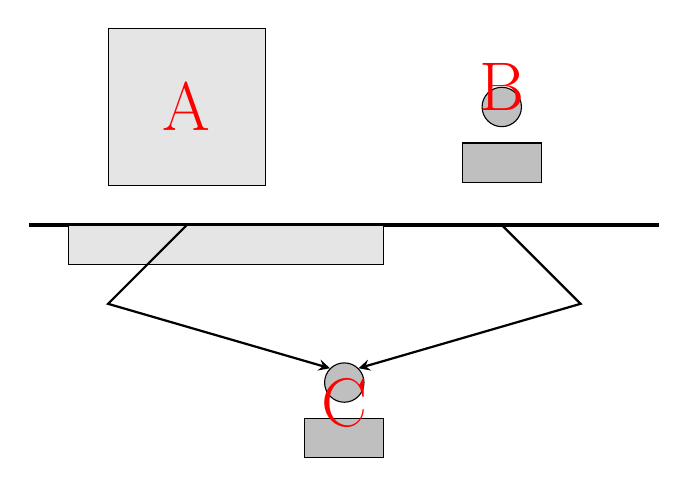
\begin{tikzpicture}[node distance=1cm, >=stealth]
        % Define components relative to a desk plane
        \draw[very thick] (-4, 0) -- (4, 0); % Desk
        
        % A (Computer) - Left side
        \draw[draw=black, fill=gray!20] (-3, 0.5) rectangle (-1, 2.5); % Monitor
        \draw[draw=black, fill=gray!20] (-3.5, -0.5) rectangle (0.5, 0); % Keyboard
        \node[font=\Huge, red] (L_A) at (-2, 1.5) {A}; 
        
        % B (Human) - Right side
        \node (B_head) at (2, 1.5) [circle, draw, fill=gray!50, minimum size=0.5cm] {};
        \draw[fill=gray!50] (B_head.south) ++(-0.5, -0.2) rectangle ++(1, -0.5);
        \node[font=\Huge, red] at (B_head.north) {B};
        
        % C (Interviewer/Judge) - Bottom center
        \node (C_head) at (0, -2) [circle, draw, fill=gray!50, minimum size=0.5cm] {};
        \draw[fill=gray!50] (C_head.south) ++(-0.5, -0.2) rectangle ++(1, -0.5);
        \node[font=\Huge, red] at (C_head.south) {C};
        
        % Communication lines (responses from A and B channeled to C)
        \draw[arrow, thick] (-2, 0) -- ++(-1, -1) -- (C_head.north west);
        \draw[arrow, thick] (2, 0) -- ++(1, -1) -- (C_head.north east);

    \end{tikzpicture}
    \caption{Conceptual setup of the Turing Test}
\end{figure}

\subsubsection{Turing's Six Primitives}
Alan Turing wrote about the six basic operations, or primitives, that are necessary to define a computational system, forming the theoretical basis of a software language (Turing Machine):

\begin{itemize}
    \item \textbf{Right:} Move the machine's head one square to the right on the tape.
    \item \textbf{Left:} Move the machine's head one square to the left on the tape.
    \item \textbf{Print:} Print a symbol on the current square.
    \item \textbf{Scan:} Identify the symbol currently on the square.
    \item \textbf{Erase:} Erase any symbols presented on the current square.
    \item \textbf{Nothing/Halt:} Stop execution; do nothing further.
\end{itemize}

\begin{figure}[H]
    \centering
    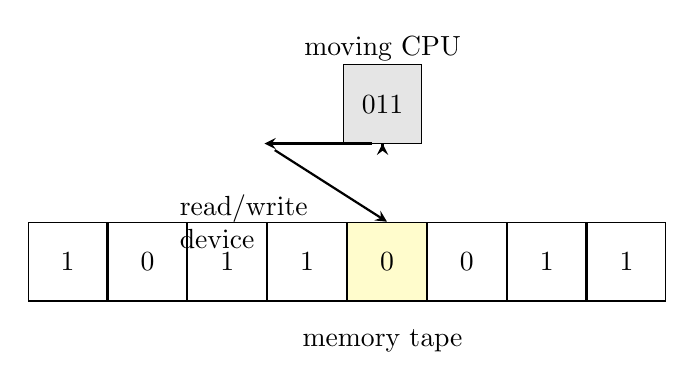
\begin{tikzpicture}[node distance=0cm, box/.style={draw, rectangle, minimum width=1cm, minimum height=1cm, align=center}]
        \node (CPU) [box, fill=gray!20] at (0, 2) {011};
        \node (CPU_label) at (0, 2.7) {moving CPU};
        
        % Tape cells
        \node (Tape1) [box] at (-4, 0) {1};
        \node (Tape2) [box, right=of Tape1] {0};
        \node (Tape3) [box, right=of Tape2] {1};
        \node (Tape4) [box, right=of Tape3] {1};
        \node (Tape5) [box, right=of Tape4, fill=yellow!20] {0}; % Current square
        \node (Tape6) [box, right=of Tape5] {0};
        \node (Tape7) [box, right=of Tape6] {1};
        \node (Tape8) [box, right=of Tape7] {1};
        
        \node (Tape_label) at (0, -1) {memory tape};
        
        % Arrow representing read/write head movement
        \draw[arrow] (CPU.south) -- (0, 1.5) node (Mid) {};
        \draw[arrow] (Mid) -- (-1.5, 1.5) node (ReadWrite) {};
        
        % Head pointing to the current square (Tape 5)
        \draw[arrow] (ReadWrite) -- (Tape5.north) node[left, xshift=-0.5cm, text width=2cm] {read/write device};
        
    \end{tikzpicture}
    \caption{Turing Machine Head Interaction with Memory Tape}
\end{figure}

\section{Modern Cryptography}

\subsection{Symmetric Encryption}
Symmetric encryption uses a single, shared secret key for both encrypting the plaintext into ciphertext and decrypting the ciphertext back into plaintext. While extremely efficient for high-volume data, the main challenge lies in securely distributing this shared key.

\begin{figure}[H]
    \centering
    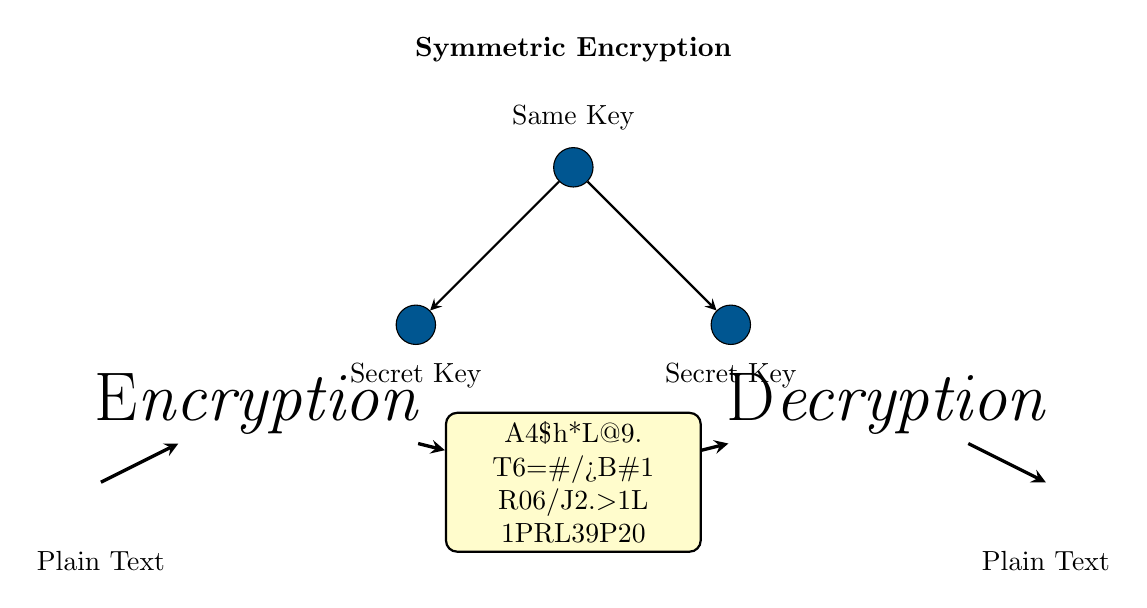
\begin{tikzpicture}[node distance=2.5cm, keyLarge/.style={circle, draw, minimum size=0.5cm, fill=ocu_blue}]
        \node (E_icon) at (1.5, -0.5) {\Huge E\textit{ncryption}};
        \node (D_icon) at (9.5, -0.5) {\Huge D\textit{ecryption}};

        \node (Key_middle) [keyLarge] at (5.5, 2.5) {};
        \node (Key_middle_label) [above=0.1cm of Key_middle] {Same Key};
        
        \node (Key1) [keyLarge] at (3.5, 0.5) {};
        \node (Key2) [keyLarge] at (7.5, 0.5) {};
        
        \node (PT1_label) at (-0.5, -2.5) {Plain Text};
        \node (CT_box) [block, text width=3cm, fill=yellow!20] at (5.5, -1.5) {A4\$h*L@9.\\T6=\#/>B\#1\\R06/J2.\textgreater 1L\\1PRL39P20};
        \node (PT2_label) at (11.5, -2.5) {Plain Text};

        % Connect keys
        \draw[arrow] (Key_middle) -- (Key1) node[below=0.1cm of Key1] {Secret Key};
        \draw[arrow] (Key_middle) -- (Key2) node[below=0.1cm of Key2] {Secret Key};
        
        % Flow
        \draw[arrow, very thick] (-0.5, -1.5) -- (E_icon);
        \draw[arrow, very thick] (E_icon) -- (CT_box);
        \draw[arrow, very thick] (CT_box) -- (D_icon);
        \draw[arrow, very thick] (D_icon) -- (11.5, -1.5);
        
        \node at (5.5, 4) {\textbf{Symmetric Encryption}};
        
    \end{tikzpicture}
    \caption{Symmetric Encryption utilizes a single key for both processes.}
\end{figure}

\subsection{Diffie-Hellman Key Exchange}
The Diffie-Hellman protocol, developed conceptually by Martin Hellman and Whitfield Diffie in the late 1960s/early 1970s, is a method for securely exchanging cryptographic keys over a public channel.

The core relies on modular arithmetic and the difficulty of the Discrete Logarithm Problem. Alice and Bob publicly agree on two large prime numbers, $p$ (the modulus) and $g$ (the generator).

\begin{tcolorbox}[title=Diffie-Hellman Example (Numbers)]
\begin{center}
\begin{tabular}{ll|ll|ll}
\toprule
\multicolumn{2}{c}{\textbf{Alice}} & \multicolumn{2}{c}{\textbf{Bob}} & \multicolumn{2}{c}{\textbf{Eve (Eavesdropper)}} \\
Known & UN & Known & UN & Known & UN \\
\midrule
$p=23$ & & $p=23$ & & $p=23$ & \\
$g=5$ & & $g=5$ & & $g=5$ & \\
$a=6$ (Private) & $B$ & $b=15$ (Private) & $A$ & $A=8, B=19$ & $a, b$ \\
\midrule
\multicolumn{6}{c}{\textbf{Public Exchange (Shared values $A$ and $B$)}} \\
$A=5^6 \bmod 23 = 8$ & & $B=5^{15} \bmod 23 = 19$ & & & \\
$B=19$ (Received) & & $A=8$ (Received) & & & \\
\midrule
\multicolumn{6}{c}{\textbf{Calculating the Shared Secret ($S$)}} \\
$S=B^a \bmod 23$ & & $S=A^b \bmod 23$ & & & \\
$S=19^6 \bmod 23 = 2$ & & $S=8^{15} \bmod 23 = 2$ & & $S=?$ & \\
\bottomrule
\end{tabular}
\end{center}
The resulting Shared Secret ($S=2$) is identical for both Alice and Bob, yet Eve, only seeing $p, g, A, B$, cannot efficiently compute $S$.
\end{tcolorbox}

\subsection{Asymmetric Encryption (PKI)}
Asymmetric encryption uses distinct public and private keys. The public key encrypts data, and only the corresponding private key can decrypt it.

\begin{figure}[H]
    \centering
    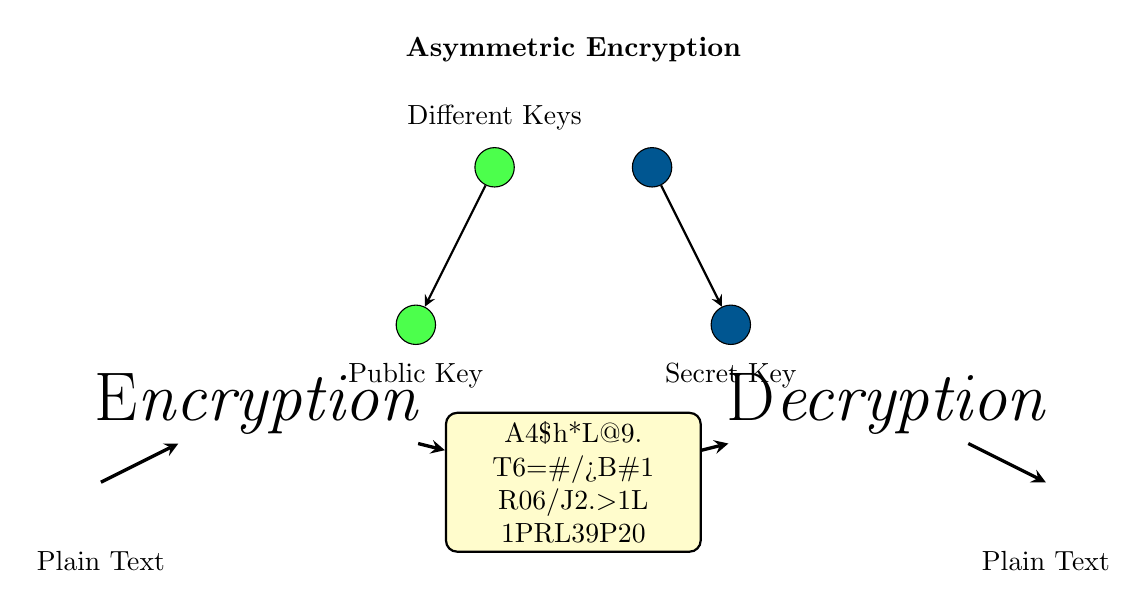
\begin{tikzpicture}[node distance=2.5cm, keyP/.style={key, minimum size=0.5cm, fill=green!70}, keyS/.style={key, minimum size=0.5cm, fill=ocu_blue}]
        \node (E_icon) at (1.5, -0.5) {\Huge E\textit{ncryption}};
        \node (D_icon) at (9.5, -0.5) {\Huge D\textit{ecryption}};

        \node (Key_middle_P) [keyP] at (4.5, 2.5) {};
        \node (Key_middle_S) [keyS] at (6.5, 2.5) {};
        \node (Key_middle_label) [above=0.1cm of Key_middle_P, text width=4cm, align=center] {Different Keys};
        
        \node (Key1) [keyP] at (3.5, 0.5) {};
        \node (Key2) [keyS] at (7.5, 0.5) {};
        
        \node (PT1_label) at (-0.5, -2.5) {Plain Text};
        \node (CT_box) [block, text width=3cm, fill=yellow!20] at (5.5, -1.5) {A4\$h*L@9.\\T6=\#/>B\#1\\R06/J2.\textgreater 1L\\1PRL39P20};
        \node (PT2_label) at (11.5, -2.5) {Plain Text};

        % Connect keys
        \draw[arrow] (Key_middle_P) -- (Key1) node[below=0.1cm of Key1] {Public Key};
        \draw[arrow] (Key_middle_S) -- (Key2) node[below=0.1cm of Key2] {Secret Key};
        
        % Flow
        \draw[arrow, very thick] (-0.5, -1.5) -- (E_icon);
        \draw[arrow, very thick] (E_icon) -- (CT_box);
        \draw[arrow, very thick] (CT_box) -- (D_icon);
        \draw[arrow, very thick] (D_icon) -- (11.5, -1.5);
        
        \node at (5.5, 4) {\textbf{Asymmetric Encryption}};
        
    \end{tikzpicture}
    \caption{Asymmetric Encryption (Public Key is used for encryption, Private Key for decryption).}
\end{figure}

\subsubsection{Certificate Authorities and PKI}
\begin{itemize}
    \item \textbf{Certificate Authorities (CA):} The primary function of a CA is to digitally sign and publicize the public key of a user. This signature affirms that the CA has verified the user's identity, establishing essential trust in online interactions.
    \item \textbf{Registration Authority (RA):} An RA assists the CA, often handling the initial identity verification and registration process before a certificate is issued.
    \item \textbf{Public Key Infrastructure (PKI):} This is the comprehensive arrangement that binds public keys to verified user identities via the CA's trusted services, enabling secure exchange.
\end{itemize}

\section{Hashing and Authentication}

\subsection{Hashing Concepts}
Hashing takes a variable-size input (such as a password) and produces a fixed-size string, known as the \textbf{hash value} or digest. Hashing is inherently \textbf{one-way}; while the calculation is deterministic, reversing the process to find the original input is computationally infeasible.

\begin{figure}[H]
    \centering
    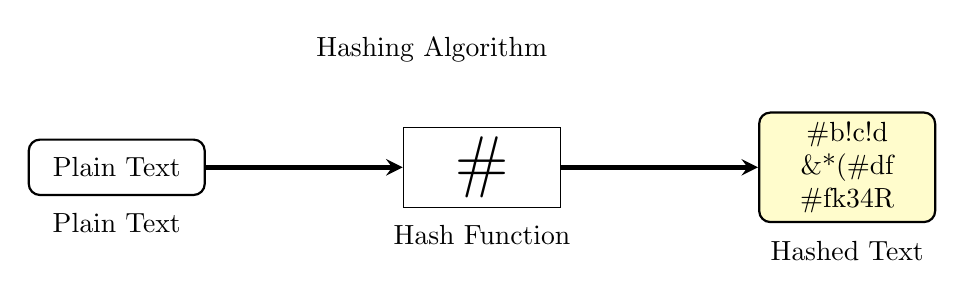
\begin{tikzpicture}[node distance=2.5cm, auto]
        \node (PT) [block, text width=2cm, fill=white] {Plain Text};
        \node (HF) [process, right=of PT, fill=white, minimum width=2cm] {\Huge \#};
        \node (HT) [block, right=of HF, text width=2cm, fill=yellow!20] {\#b!c!d\\ \&*(\#df\\ \#fk34R};
        
        \node (Alg) at (4, 1.5) {Hashing Algorithm};
        
        % Labels
        \node (PT_label) [below=0.1cm of PT] {Plain Text};
        \node (HF_label) [below=0.1cm of HF] {Hash Function};
        \node (HT_label) [below=0.1cm of HT] {Hashed Text};
        
        \draw [arrow, ultra thick] (PT) -- (HF);
        \draw [arrow, ultra thick] (HF) -- (HT);
    \end{tikzpicture}
    \caption{The Hashing Process}
\end{figure}

\subsection{Salting}
A \textbf{Salt} is defined as a sequence of random bits that is cryptographically combined with the input (password) before the hashing function is applied.

\begin{itemize}
    \item \textbf{Function:} Salting ensures that even if two users choose the exact same password, their respective hashed password will be unique because the random salt value differs.
    \item \textbf{Defense:} Salting significantly complicates offline password attacks such as dictionary attacks and rainbow table attacks, as the attacker cannot pre-calculate hashes for common words.
\end{itemize}

\subsection{Hashing Methods}
\begin{itemize}
    \item \textbf{Secure Hash Algorithm (SHA):} The most widely used family of hash functions. Versions include SHA-1 (now deprecated), SHA-2 (SHA-256 and SHA-512), and the latest standard, SHA-3.
    \item \textbf{MD5 (Message-Digest Algorithm 5):} An older algorithm now considered cryptographically weak because it is \textbf{not collision resistant}, meaning it is possible (though difficult) to find two different inputs that yield the same hash output.
    \item \textbf{RACE Integrity Primitives Evaluation Message Digest (RIPEMD):} A standardized hash function often used in European contexts.
\end{itemize}

\subsection{Steganography}
Steganography is distinct from cryptography. It is the art and science of writing hidden messages in such a way that no observer suspects the existence of the message at all. The communication is concealed within an ordinary file (e.g., a digital picture or audio file), ensuring the messages do not attract attention to themselves.

\section{Social Engineering Attacks}

Social engineering is the psychological manipulation of people into performing actions or divulging confidential information.

\subsection{Social Engineering Techniques}
Attacks rely on psychological triggers, including:
\begin{itemize}
    \item \textbf{Commitment:} Exploiting a victim's desire to appear consistent after making an initial small promise, obligating them to fulfill larger requests later. \textbf{Conformity} is a special type, leveraging implied social commitment.
    \item \textbf{Authority:} Assuming a role of authority (e.g., a technical manager) that the attacker does not actually possess, leveraging the victim's deference to power.
    \item \textbf{Reciprocation:} Offering an unsolicited gift or favor, creating a social pressure to return the favor by granting access or information.
    \item \textbf{Likening:} Behaving in a way that appears similar to a member of a trusted group (e.g., political or religious organizations) to build rapport and confidence.
    \item \textbf{Scarcity:} Introducing the perception that an item or opportunity is rare or limited in time, increasing its perceived value and compelling the victim to rush their decision-making. The tactic of applying severe time constraints is known as \textbf{Rushing}.
\end{itemize}

\subsection{Authority: The Three Types}
The authority technique manifests in three ways:
\begin{enumerate}
    \item \textbf{Impersonation:} Directly pretending to be a person of authority (like a system administrator).
    \item \textbf{Diffusion of Responsibility:} Manipulating a decision from an individual process to a collective one, leading to less scrutiny by any single person.
    \item \textbf{Reciprocation:} As described above, using favors to create obligation.
\end{enumerate}

\subsection{Reverse Social Engineering (RSE)}
RSE is a unique attack where the attacker tricks the victim into asking the attacker for assistance, thereby placing the attacker in the trusted position of solving a problem. RSE involves three phases:
\begin{enumerate}
    \item \textbf{Sabotage:} The attacker creates a problem (e.g., a system error) compelling the victim to seek a solution.
    \item \textbf{Advertise:} The attacker advertises their willingness and ability to solve the exact problem they created.
    \item \textbf{Assist:} When asked for help, the attacker uses the assistance process to request sensitive data (like passwords) or access to the system.
\end{enumerate}

\subsection{Social Engineering Defenses}
The most effective defense against social engineering attacks is robust \textbf{EDUCATION}. This should be reinforced by:
\begin{itemize}
    \item \textbf{Training:} Regular, repeated training ensures employees retain knowledge of current threats.
    \item \textbf{Reaction:} Teaching employees to recognize an attack attempt and immediately move to an alert state.
    \item \textbf{Inoculation:} Making attack resistance and verification procedures a normal, expected, and habitual part of the work experience.
\end{itemize}

\subsection{Physical Security Attacks}
Attacks that exploit human psychology and physical presence:
\begin{itemize}
    \item \textbf{Tailgating:} Seeking entry to a restricted area immediately following an authorized person without presenting credentials.
    \item \textbf{Shoulder Surfing:} Covertly observing a user type their password or read confidential information from their screen.
    \item \textbf{Leaving Computer Unlocked:} A failure of basic security hygiene, allowing unauthorized access to an active session (The mantra is: \textbf{TRUST NO ONE}).
\end{itemize}

\section{Personally Identifiable Information (PII) and Phishing}

\subsection{PII Targets}
Attackers target \textbf{Personally Identifiable Information (PII)}, which can be used to impersonate, defraud, or steal identity. Key categories include:
\begin{itemize}
    \item \textbf{Name:} Full name, maiden name, mother's maiden name.
    \item \textbf{Personal Identification Numbers:} Social Security Number (SSN), Passport Number, Drivers License Number, Taxpayer ID.
    \item \textbf{Personal Address:} Street address, city, state, ZIP code.
    \item \textbf{Personal Phone \#/Email.}
    \item \textbf{Personal Characteristics:} Photograph, fingerprints, handwriting.
    \item \textbf{Biometric Data:} Retina scans, voice signatures, facial geometry.
    \item \textbf{Financial Data:} Bank accounts, credit cards, tax records.
\end{itemize}
Other shared PII includes Date/Place of Birth, Race, Religion, Employment, Medical, and Education Information.

\subsection{Phishing and its Variants}
Phishing is the fraudulent attempt to obtain sensitive information (usernames, passwords, bank account info) by posing as a legitimate entity.

\begin{itemize}
    \item \textbf{Spear Phishing:} Directed at specific individuals or small groups, requiring research into the target.
    \item \textbf{Whaling:} A form of spear phishing targeting senior executives or high-profile individuals (e.g., CEOs like Jeff Bezos).
    \item \textbf{Vishing:} Phishing conducted via voice call (VoIP or telephone).
    \item \textbf{Smishing:} Phishing conducted via SMS or text message.
\end{itemize}

\subsection{HIPAA}
The \textbf{Health Insurance Portability and Accountability Act (HIPAA)} of 1996 is a crucial piece of legislation designed to protect the privacy and security of certain health information in the United States.

\subsection{Multi-Factor Authentication (MFA)}
MFA is an authentication method that requires the user to successfully present two or more pieces of evidence (factors) to an authentication mechanism.

\begin{figure}[H]
    \centering
    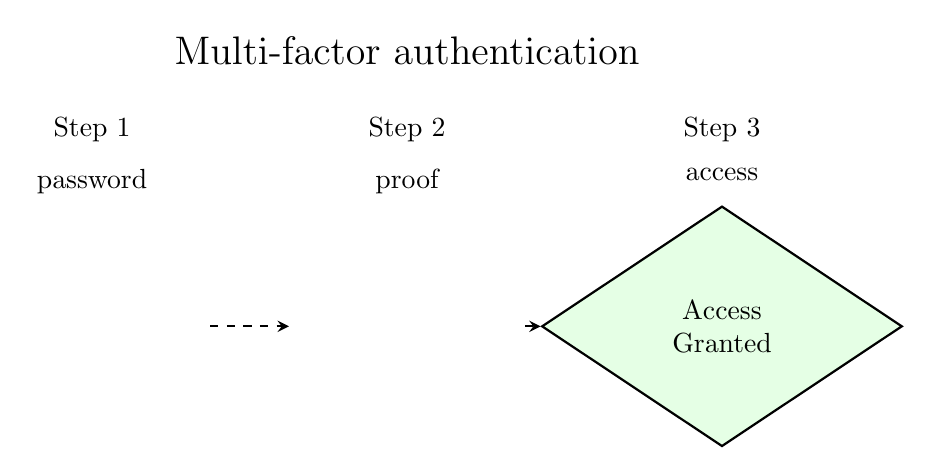
\begin{tikzpicture}[node distance=3cm, >=stealth]
        % Step 1: Password
        \node (S1_label) at (0, 3) {Step 1};
        \node (S1_text) [below=0.1cm of S1_label] {password};
        
        % Step 2: Proof
        \node (S2_label) at (4, 3) {Step 2};
        \node (S2_text) [below=0.1cm of S2_label] {proof};
        
        % Step 3: Access
        \node (S3_label) at (8, 3) {Step 3};
        \node (S3_text) [below=0.1cm of S3_label] {access};
        
        \node (Access) [decision, draw, thick, fill=green!10, text width=3cm, aspect=1.5] at (8, 0.5) {Access\\ Granted};
        
        % Flow arrows
        \draw[arrow, thick, dashed] (1.5, 0.5) -- (2.5, 0.5);
        \draw[arrow, thick, dashed] (5.5, 0.5) -- (Access.west);
        
        \node at (4, 4) {\Large Multi-factor authentication};
    \end{tikzpicture}
    \caption{Conceptual flow of Multi-factor Authentication}
\end{figure}

\section{Password Attacks and Malware}

\subsection{Dictionary and Brute-Force Attacks}
A \textbf{Dictionary Attack} is a type of brute-force cyberattack that utilizes pre-compiled lists of common words, leaked passwords, or common keyboard patterns to try to gain access.

More advanced attack types include:
\begin{itemize}
    \item \textbf{Rule-based Attack:} Applies modifications to dictionary words (e.g., substituting 'a' with '4' or 'o' with '0') based on known user habits, drastically increasing the chance of success against common password patterns.
    \item \textbf{Mask Attack:} An optimized brute-force search that reduces computation time by exploiting known information about the password's format or length, often defining specific character sets for unknown positions.
\end{itemize}

\subsection{Malware Types}
\begin{itemize}
    \item \textbf{Virus:} Malware that must attach itself to a host program and requires human interaction (e.g., execution of the host file) to replicate and spread.
    \item \textbf{Worm:} Malware that is self-replicating and can spread autonomously across a network without requiring any human interaction.
    \item \textbf{Logic Bomb:} A set of malicious instructions secretly incorporated into a program, designed to execute a payload only when a specific condition (a logical trigger) is met.
    \item \textbf{Backdoor:} A clandestine method of bypassing standard authentication or encryption measures, typically left by a developer or attacker for future covert access.
    \item \textbf{Trojan Horse:} A program that appears benign or useful but contains hidden malicious intent. Typical actions include downloading harmful software, installing keyloggers, deleting files, or opening a backdoor.
    \item \textbf{Ransomware:} A payload (often a virus) that locks down the user's files (usually via strong encryption) and demands a ransom payment (often cryptocurrency) for the key. Unpatched systems are highly vulnerable to ransomware exploits.
\end{itemize}

\section{Networking Fundamentals}

\subsection{The Open Systems Interconnect (OSI) Model}
The OSI Model is a conceptual framework used to describe the function of a networking system using seven layers.

\begin{longtable}{p{2cm} p{7cm} p{4.5cm}}
\toprule
\rowcolor{table_header} \textbf{Layer} & \textbf{Description} & \textbf{Protocols} \\
\midrule
\endhead
\multicolumn{3}{c}{\textit{...Continued on next page}} \\
\endfoot
\bottomrule
\endlastfoot
Application & This layer interfaces directly to applications and performs common application services for the processes (e.g., email, web browsing). & POP, SMTP, DNS, FTP, Telnet \\
Presentation & The presentation layer handles data formatting, ensuring that data transmitted across the network is comprehensible to the receiving system. It also manages encryption and compression. & Telnet, NDR, LPP \\
Session & Manages the dialogue and synchronization between two communicating applications, establishing and terminating connections (sessions). & NetBIOS \\
Transport & Provides reliable or unreliable end-to-end communication control, managing segmentation, reassembly, and error recovery. & TCP (Reliable), UDP (Unreliable) \\
Network & This crucial layer handles routing and logical addressing (IP addresses), determining the optimal path for data packets across interconnected networks. & IP, ARP, ICMP \\
Data link & Handles the logical organization of data bits into frames. It is divided into two sublayers: the Media Access Control (MAC) and the Logical Link Control (LLC). & SLIP, PPP \\
Physical & Describes the physical properties of the transmission media and electrical signaling characteristics (voltage levels, cable types, connectors). & IEEE 1394, DSL, ISDN \\
\end{longtable}
\tcbset{colback=red!5, colframe=red!40}
\begin{tcolorbox}
\textbf{Warning:} Please Do Not Tell Secret Passwords Anytime (A common mnemonic for remembering the layer order: Please Do Not Tell Secret Passwords Anytime $\rightarrow$ Physical, Data Link, Network, Transport, Session, Presentation, Application).
\end{tcolorbox}

\subsection{Network Devices}
\begin{itemize}
    \item \textbf{Router (Layer 3):} Forwards data packets along networks based on logical IP addresses. It is connected to at least two networks (LANs or WANs).
    \item \textbf{Switch (Layer 2):} Filters and forwards data packets between LAN segments based on unique MAC addresses, directing traffic only to the intended recipient device.
    \item \textbf{Hub (Layer 1):} A basic connection point that connects network segments. It broadcasts all incoming data to all connected devices, leading to high network congestion.
\end{itemize}

\subsection{IP and MAC Addresses}
\begin{itemize}
    \item \textbf{IPv4:} A 32-bit address represented as four three-digit numbers separated by periods (e.g., 107.22.98.129). Each octet ranges from 0 to 255.
    \item \textbf{IPv6:} A 128-bit address using hexadecimal numbering (e.g., 3FFE:B000:800:2:C).
    \item \textbf{IP Ranges (First Byte):} Class A (0-126), Class B (128-191), Class C (192-223), Class D (224-247, Multicasting), Class E (248-255, Experimental).
    \item \textbf{Private Networks (RFC 1918):} 10.0.0.0--10.255.255.255; 172.16.0.0--172.31.255.255; 192.168.0.0--192.168.255.255.
    \item \textbf{Local Host (localhost):} 127.0.0.1.
    \item \textbf{MAC Addresses:} Unique six-byte hexadecimal hardware addresses burned into every NIC. The \textbf{Address Resolution Protocol (ARP)} converts IP addresses to MAC addresses for local network communication.
\end{itemize}

\subsection{Protocols and Ports}
\begin{center}
\begin{tabular}{lr}
\toprule
\rowcolor{table_header} \textbf{Protocol} & \textbf{Port} \\
\midrule
FTP & 20, 21 \\
SSH & 22 \\
Telnet & 23 \\
SMTP & 25 \\
DNS & 53 \\
HTTP & 80 \\
POP3 & 110 \\
LDAP & 389 \\
HTTPS & 443 \\
RDP & 3389 \\
\bottomrule
\end{tabular}
\end{center}

\subsection{Basic Network Utilities}
\begin{itemize}
    \item \textbf{ipconfig (Windows) / ifconfig (Mac/Unix):} Displays network configuration, including IP address, subnet mask, and gateway.
    \item \textbf{ping:} Uses ICMP packets to test connectivity and measure round-trip time to a remote host.
    \item \textbf{tracert (Windows) / traceroute (Unix):} Traces the route a packet takes to a destination, listing all intermediate routers (hops).
    \item \textbf{netstat:} Displays active network connections, listening ports, and usage statistics. Use `netstat -an` (Windows) or `netstat -an | grep LISTEN` (Unix/Bash) to check for open ports.
\end{itemize}

\subsection{UDP vs. TCP}
\begin{itemize}
    \item \textbf{UDP (User Datagram Protocol):} Connection-less, faster, sends packets in chunks (datagrams). Less reliable as delivery is not guaranteed.
    \item \textbf{TCP (Transmission Control Protocol):} Connection-oriented, establishes a session handshake, provides bidirectional communication, and is more reliable due to error checking and guaranteed delivery.
\end{itemize}

\section{Denial of Service (DoS) Attacks}

\subsection{Denial of Service (DoS)}
A DoS attack aims to exhaust system resources, making a service unavailable by overwhelming it with traffic, often utilizing the `ping` utility.

\begin{figure}[H]
    \centering
    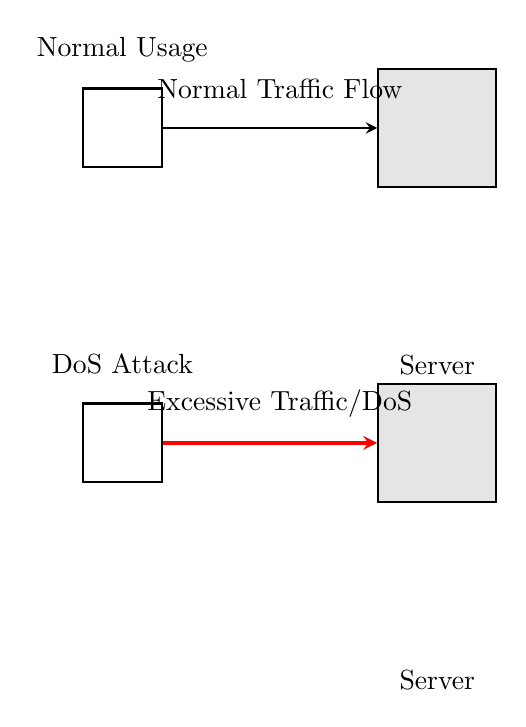
\begin{tikzpicture}[node distance=2cm, auto, thick]
        % Normal Usage
        \node (N_label) at (-3, 5.5) {Normal Usage};
        \node (N_client) [comp] at (-3, 4.5) {};
        \node (N_server) [server] at (1, 4.5) {};
        \node (N_server_label) [below=of N_server] {Server};
        \node (N_flow) [block, draw=none, fill=none] at (-1, 5) {Normal Traffic Flow};
        
        \draw[arrow] (N_client) -- (N_server);
        
        % DoS Attack
        \node (D_label) at (-3, 1.5) {DoS Attack};
        \node (D_client) [comp] at (-3, 0.5) {};
        \node (D_server) [server] at (1, 0.5) {};
        \node (D_server_label) [below=of D_server] {Server};
        \node (D_flow) [block, draw=none, fill=none] at (-1, 1) {Excessive Traffic/DoS};
        
        \draw[arrow, red, very thick] (D_client) -- (D_server);
    \end{tikzpicture}
    \caption{Normal Usage versus Denial of Service Attack}
\end{figure}

\subsection{Distributed Denial of Service (DDoS)}
A DDoS is a major variation where the attack is launched from \textbf{multiple clients} (a botnet of "zombie machines"). Because the sources are numerous and dispersed, it is significantly more difficult to track and block.

\subsection{SYN Flood}
The SYN Flood attack exploits the initial TCP handshake by sending SYN packets without completing the ACK phase, exhausting the server's connection table.

Mitigation techniques include:
\begin{itemize}
    \item Micro Blocks (temporarily blocking source IPs).
    \item Bandwidth Throttling.
    \item SYN Cookies (a method to delay state allocation until the handshake is verified).
    \item RST Cookies (sending an immediate RST).
    \item Stack Tweaking (optimizing server connection handling).
\end{itemize}

\subsection{Smurf Attack}
This attack uses ICMP requests directed at a network's broadcast address with the victim's IP address spoofed as the source. All network devices then flood the victim with echo replies.

\subsection{Ping of Death (PoD)}
PoD attacks target vulnerable systems by sending ICMP packets larger than 65,535 bytes. This causes older systems to crash upon reassembly. Modern systems prevent this by automatically dropping oversized packets.

\subsection{Reflection Attacks}
\begin{itemize}
    \item \textbf{UDP Flood and ICMP Flood:} The UDP flood is a variation of PoD targeting random open ports. ICMP flood is synonymous with the ping flood.
    \item \textbf{Distributed Reflection DoS (DRDoS):} This attack uses \textbf{routers} or other third-party servers to execute the attack. The attacker spoofs the target's IP address and sends requests to the reflectors. The large volume of responses (reflections) is directed toward the target. Routers do not need to be compromised; they just need to be configured (or misconfigured) to forward broadcast packets.
\end{itemize}

\begin{figure}[H]
    \centering
    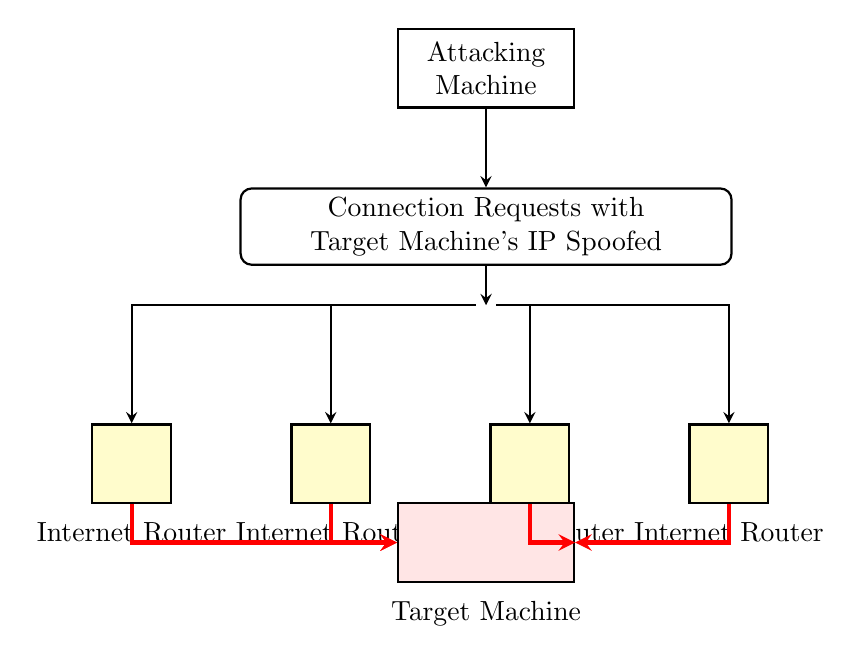
\begin{tikzpicture}[node distance=1.5cm, auto, thick,
        comp/.style={draw, rectangle, minimum size=1cm},
        router/.style={draw, rectangle, minimum size=1cm, fill=yellow!20},
        target/.style={draw, rectangle, minimum size=1cm, fill=red!10}
    ]
        \node (Attacker) [comp, text width=2cm, align=center] at (0, 4) {Attacking Machine};
        
        \node (Connection) [block, below=1cm of Attacker, text width=6cm, fill=white] {Connection Requests with \\ Target Machine's IP Spoofed};
        
        \draw[arrow] (Attacker) -- (Connection);
        
        % Routers (Reflectors)
        \node (R1) [router, below=2cm of Connection, xshift=-4.5cm] {};
        \node (R2) [router, right=of R1] {};
        \node (R3) [router, right=of R2] {};
        \node (R4) [router, right=of R3] {};

        \node[below=0.1cm of R1] {Internet Router};
        \node[below=0.1cm of R2] {Internet Router};
        \node[below=0.1cm of R3] {Internet Router};
        \node[below=0.1cm of R4] {Internet Router};
        
        % Target Machine
        \node (Target) [target, text width=2cm, below=3cm of Connection] {};
        \node (Target_label) [below=0.1cm of Target] {Target Machine};

        % Attacker -> Routers (Spoofed Source IP)
        \draw[arrow] (Connection.south) -- ++(0, -0.5) node (Mid) {} ;
        \draw[arrow] (Mid) -| (R1.north);
        \draw[arrow] (Mid) -| (R2.north);
        \draw[arrow] (Mid) -| (R3.north);
        \draw[arrow] (Mid) -| (R4.north);


        % Routers -> Target (Reflection/Attack traffic)
        \draw[arrow, red, ultra thick] (R1.south) |- (Target.west);
        \draw[arrow, red, ultra thick] (R2.south) |- (Target.west);
        \draw[arrow, red, ultra thick] (R3.south) |- (Target.east);
        \draw[arrow, red, ultra thick] (R4.south) |- (Target.east);
        
    \end{tikzpicture}
    \caption{Distributed Reflection DoS (DRDoS) Attack Flow}
\end{figure}

\section{Risk Assessment and Security Management}

\subsection{Loss Expectancy Calculations}

\subsubsection{Single Loss Expectancy (SLE)}
The SLE calculates the expected monetary impact resulting from a single occurrence of a threat.
\begin{itemize}
    \item $\text{SLE} = \text{Asset Value (AV)} \times \text{Exposure Factor (EF)}$
    \item The Exposure Factor (EF) is the percentage of the asset's value that is expected to be lost if a specific threat materializes.
\end{itemize}
\textbf{Example:} If an asset has an AV of \$800, and the estimated loss (EF) is 90\% (0.9), the SLE is $\$800 \times 0.9 = \$720$.

\subsubsection{Annualized Loss Expectancy (ALE)}
The ALE provides the expected financial loss over a one-year period.
\begin{itemize}
    \item $\text{ALE} = \text{SLE} \times \text{Annual Rate of Occurrence (ARO)}$
    \item The ARO is the estimated frequency with which the loss event will occur within a year.
\end{itemize}
\textbf{Example:} If the SLE is \$720 and you estimate an ARO of 6 (six laptops lost annually), the ALE is $\$720 \times 6 = \$4320$.

\subsection{Evaluating Security Risk}
Risk (R) is evaluated by assessing the relative strengths of attractiveness, information content, and existing security controls. Each factor is typically scored on a 1 to 10 scale.
\begin{itemize}
    \item $\text{Attractiveness (A)}:$ Desirability of the asset to attackers.
    \item $\text{Information (I)}:$ Sensitivity and inherent value of the data.
    \item $\text{Security (S)}:$ Effectiveness and implementation of current safeguards.
\end{itemize}
\textbf{Formula:} $\text{Rating (R)} = (\text{A} + \text{I}) - \text{S}$. A lower final rating (R) indicates a more secure system.

\subsection{The Six P's of Assessment}
For comprehensive security auditing and risk management, six key areas must be assessed:
\begin{enumerate}
    \item Patches
    \item Ports
    \item Protect
    \item Physical
    \item Probe
    \item Policies
\end{enumerate}

\subsubsection{(1) Patches}
A mandatory \textbf{Patch Policy} must be written and strictly followed. All applications and operating systems requiring security updates must be checked regularly. This step should always be the first on any system assessment list. Automated patch systems commonly used include Windows Update, HFNetChkPro, and McAfee ePolicy Orchestrator.

\subsubsection{(2) Ports}
Since specific ports are often targeted by virus attacks, closing all unused network ports is critical to reduce the attack surface and vulnerability profile.

\subsubsection{(3) Protect}
Protection mechanisms must be rigorously assessed for functionality and placement. This includes ensuring effective deployment of:
\begin{itemize}
    \item Firewalls
    \item Antivirus and Antispyware software
    \item Intrusion Detection Systems (IDS)
    \item Proxy servers or Network Address Translation (NAT) devices
    \item Data transmission encryption
\end{itemize}

\subsubsection{(4) Physical}
Physical security controls must restrict access to sensitive locations, including server rooms, workstations, miscellaneous equipment, and data backup media. Strategies include:
\begin{itemize}
    \item Biometric locks.
    \item Strict visitor logging and mandatory escorting.
    \item Inspection of all bags.
    \item Prohibiting unauthorized portable devices (e.g., flash drives) that could record data.
    \item Logging and tracking all printing and copying.
\end{itemize}

\subsubsection{(5) Probe}
Probing involves actively searching for weaknesses, encompassing three main methodologies:
\begin{itemize}
    \item \textbf{Port Scanning:} Systematically checking well-known and custom ports to identify which are open (listening).
    \item \textbf{Enumerating:} Attempting to determine the active resources on the target network, such as user accounts, shared drives, and printers.
    \item \textbf{Vulnerability Assessment:} Using automated tools or manual inspection to seek out known vulnerabilities based on public databases.
\end{itemize}

Key vulnerability lists and standards include:
\begin{itemize}
    \item \textbf{Common Vulnerabilities and Exposures (CVE):} Maintained by the Mitre Corporation, providing unique identifiers for public security flaws.
    \item \textbf{National Institute of Standards and Technology (NIST):} Utilizes the CVE format in its extensive security documentation.
    \item \textbf{Open Web Application Security Project (OWASP):} Provides security standards for web applications and publishes the influential Top 10 list of critical risks.
\end{itemize}

\subsubsection{(6) Policies - The McCumber Cube}
The McCumber Cube is a foundational model for defining Information Assurance goals and methods.

\begin{tcolorbox}[title=The McCumber Cube Dimensions]
The cube defines security based on the intersection of three dimensions:
\begin{itemize}
    \item \textbf{Goals (CIA Triad):} Confidentiality, Integrity, Availability.
    \item \textbf{Information States:} Storage, Transmission, Processing.
    \item \textbf{Safeguards (Countermeasures):} Policy and Practices, Human Factors, Technology.
\end{itemize}
\end{tcolorbox}

Security documentation ensures compliance and recoverability. Essential documents include:
\begin{itemize}
    \item \textbf{Physical Security Documentation:} Lists all controls in place, device locations, keys/access lists for locked rooms, and entry logs.
    \item \textbf{Policy and Personnel Documentation:} Filed copies of all security policies, revisions, signed copies of user awareness agreements, and lists of personnel access rights.
    \item \textbf{Probe Documents:} Internal and external audit results, follow-up reports detailing flaw correction, and documentation of all security incidents and remediation steps.
    \item \textbf{Network Protection Documents:} Detailed configuration of firewalls and IDS, usage documentation for antivirus/antispyware, records of honeypots in use, and individual machine security measures.
\end{itemize}

\section{Security Professionals and Attacks}

\subsection{Types of Hackers}
\begin{itemize}
    \item \textbf{White Hat Hacker (Penetration Tester):} Someone authorized to simulate a cyber attack on a target system with the owner's permission to improve security posture.
    \item \textbf{Black Hat Hacker (Cracker):} A malicious individual who gains unauthorized access to cause harm, steal information, or disrupt services.
    \item \textbf{Gray Hat Hacker:} Individuals who may violate laws (e.g., hacking without permission) but often lack malicious intent, sometimes reporting vulnerabilities publicly without seeking compensation or authorization first.
\end{itemize}

A \textbf{Penetration Tester} or \textbf{Ethical Hacker} is an authorized security professional (often a company or security firm) who performs several attacks on an organization and provides a comprehensive report detailing vulnerabilities and how to fix them.

\subsection{The Evil Twin Attack}
An \textbf{Evil Twin} is a fraudulent Wi-Fi access point configured to appear legitimate, often mirroring the Service Set Identifier (SSID) of a trusted public network. It is set up to eavesdrop on wireless communications. The evil twin is effectively the wireless LAN equivalent of a phishing scam, tricking users into connecting to a compromised network.

\

\end{document}
